\documentclass[11pt]{beamer}
\usetheme[
  %%% options passed to the outer theme
  progressstyle=fixedCircCnt,   %either fixedCircCnt, movCircCnt, or corner
    rotationcw,          % change the rotation direction from counter-clockwise to clockwise
    shownavsym          % show the navigation symbols
  ]{AAUsimple}

\definecolor{darkblue}{RGB}{51,51,179}

% If you want to change the colors of the various elements in the theme, edit and uncomment the following lines
% Change the bar and sidebar colors:
\setbeamercolor{AAUsimple}{fg=gray!50 ,bg=darkblue}
\setbeamercolor{sidebar}{bg=gray!20}
\setbeamercolor{frametitle}{fg=darkblue!5,bg=darkblue}
% Change the color of the structural elements:
\setbeamercolor{structure}{fg=darkblue}
% Change the frame title text color:
%\setbeamercolor{frametitle}{fg=darkblue!20}
% Change the normal text color background:
%\setbeamercolor{normal text}{fg=black,bg=gray!10}
% ... and you can of course change a lot more - see the beamer user manual.

\usepackage[utf8]{inputenc}
\usepackage[spanish]{babel}
\usepackage[T1]{fontenc}
% Or whatever. Note that the encoding and the font should match. If T1
% does not look nice, try deleting the line with the fontenc.
\usepackage{helvet}

% colored hyperlinks
\newcommand{\chref}[2]{%
  \href{#1}{{\usebeamercolor[bg]{AAUsimple}#2}}%
}

\title{Control automático del proceso de fermentación de vino usando la CIAA}

\subtitle{Presentación del Trabajo Final}  % could also be a conference name

\date{\today}

\author{ Ing. Luis Enrique Chico Capistrano }

% - Give the names in the same order as they appear in the paper.
% - Use the \inst{?} command only if the authors have different
%   affiliation. See the beamer manual for an example

\institute[
  %  {\includegraphics[scale=0.2]{aau_segl}}\\ %insert a company, department or university logo
  Dept.\ de electrónica\\
  Facultad de Ingeniería\\
  Universidad de Buenos Aires
] % optional - is placed in the bottom of the sidebar on every slide
{% is placed on the bottom of the title page
  Carrera de Especialización en Sistemas Embebidos\\
  Facultad de Ingeniería\\
  Universidad de Buenos Aires

  %there must be an empty line above this line - otherwise some unwanted space is added between the university and the country (I do not know why;( )
}

% specify a logo on the titlepage (you can specify additional logos an include them in 
% institute command below
\pgfdeclareimage[height=1.5cm]{titlepagelogo}{imagenes/logo_facu_circle} % placed on the title page
%\pgfdeclareimage[height=1.5cm]{titlepagelogo2}{AAUgraphics/aau_logo_new} % placed on the title page
\titlegraphic{% is placed on the bottom of the title page
  \pgfuseimage{titlepagelogo}
  %  \hspace{1cm}\pgfuseimage{titlepagelogo2}
}

\definecolor{darkblue}{RGB}{51,51,179}
\setbeamercolor{bgcolor}{fg=white,bg=darkblue}


\newcommand\Wider[2][3em]{%
  \makebox[\linewidth][c]{%
    \begin{minipage}{\dimexpr\textwidth+#1\relax}
      \raggedright#2
    \end{minipage}%
  }%
}

\beamerdefaultoverlayspecification{<+->}

\AtBeginSection[]
{
  \begin{frame}<beamer>
    \frametitle{\textbf{\LARGE{Agenda}}}
    \fontsize{18pt}{18}\selectfont
    \tableofcontents[currentsection]
  \end{frame}
}

\begin{document}
\begin{frame}[plain,noframenumbering]
  \begin{center}
    \vspace{5px}	
    \large\textbf{Carrera de Especialización en Sistemas Embebidos}\\
    \vspace{5px}
    \Large\textbf{Presentación de Trabajo Final}\\
    \vspace{10px}
    \hspace{-20px}
      \begin{beamercolorbox}[center,dp=2ex,ht=.22\textheight, wd=1\paperwidth]{bgcolor}
        \large\textbf{Control automático del proceso de fermentación de vino usando la CIAA}\\
          \vspace{5px}
        \large{Ing. Luis Enrique Chico Capistrano}
        %\texttt{lchico@fi.uba.ar}
      \end{beamercolorbox}
    \hfill
    \vspace{5px}
    %\vfill
    \begin{minipage}[t]{0.75\textwidth}
      \begin{flushleft} \large
        \hspace{-20px}
        \textbf{Director:}\\
        \vspace{5px}
        Ing. Juan Manuel Cruz\\
        \vspace{5px}
        \hspace{-20px}
        \textbf{Jurados:} \\
        \vspace{5px}
        Dr. Ing. Pablo Gomez (FIUBA) \\
        Esp. Ing. Franco Bucafusco (CESE)\\
        Esp. Ing. Sergio De Jesús Meleán (CESE)\\
      \end{flushleft}
    \end{minipage}
    \begin{minipage}[t]{0.2\textwidth}
      \vspace{12px}
      \begin{flushright} \large
        \vfill
        \begin{figure}[H]
          
\includegraphics[width=2cm]{./imagenes/logo_facu_circle}
        \end{figure}	
      \end{flushright}
    \end{minipage}
      \end{center}
\end{frame}


% TOC
\begin{frame}{\textbf{\LARGE{Agenda}}}
  \fontsize{18pt}{18}\selectfont
  \tableofcontents
\end{frame}
%%%%%%%%%%%%%%%%

\section{Motivación}
\begin{frame}{\textbf{\LARGE{¿Porqué realizar este proyecto?}}}
  \fontsize{18pt}{18}\selectfont
  \vspace{-30px}
  \begin{itemize}
    \item Satisfacer las necesidades de la bodega Chico Zossi.
      \vspace{5px}
    \item Implementar en un microcontrolador un sistema de control con interfaz web.
      \vspace{5px}
    \item Trabajar con la plataforma CIAA.
  \end{itemize}
\end{frame}

\section{Introducción}

\begin{frame}{\textbf{\LARGE{¿Cómo se elabora el vino?}}}
  \fontsize{18pt}{18}\selectfont
  \hspace{-40px}
  \vspace{-30px}
  \begin{figure}[H]
    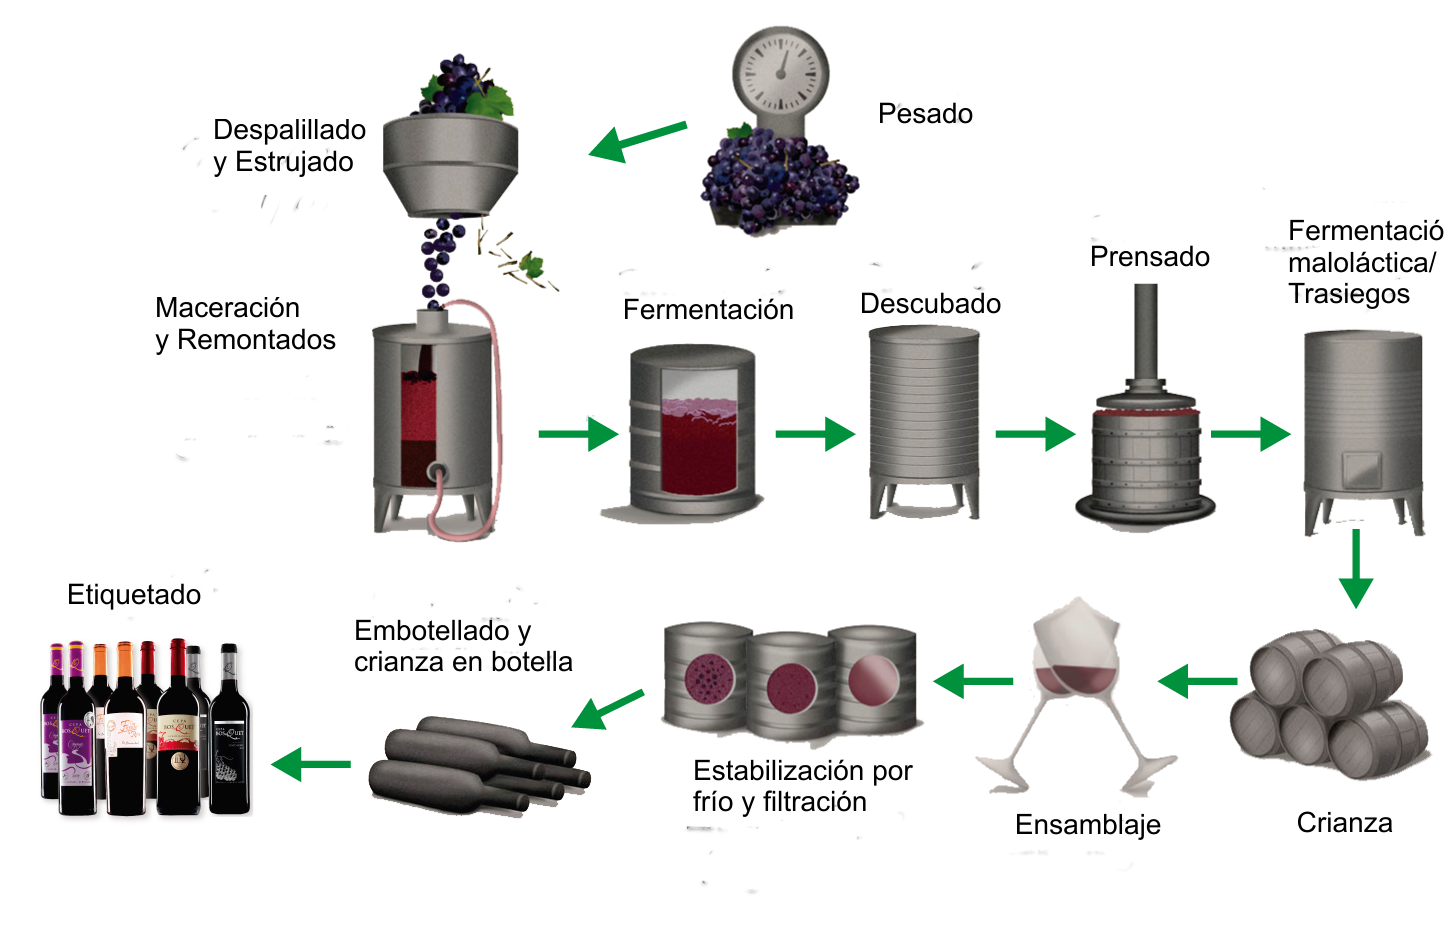
\includegraphics[width=1\textwidth]{./imagenes/elaboracion-del-vino-tinto.png}
  \end{figure}	  	  	
\end{frame}

\begin{frame}{\LARGE{\textbf{Proceso de Fermentación}}}
  \fontsize{18pt}{18}\selectfont
  \vspace{-30px}
  \begin{itemize}
      \vspace{15px}
    \item Vinos Tintos
      \vspace{5px}
      \begin{itemize}
        \item Tiempo de fermentación: 6 a 12 dias
        \vspace{5px}
        \item Temperatura de fermentación: $20^o\ a\ 24^oC$
      \end{itemize}
        \vspace{15px}
      \item Vinos Blancos
        \vspace{5px}
        \begin{itemize}
          \item Tiempo de fermentación: 5 a 15 dias
          \vspace{5px}
          \item Temperatura de fermentación: $10^o\ a\ 15^oC$
        \end{itemize}
  \end{itemize}	
\end{frame}


\section[Problema]{Condiciones actuales}

\begin{frame}{\textbf{\LARGE{Condiciones actuales}}}
  \fontsize{18pt}{18}\selectfont
  \begin{itemize}
    \item { Dificultad para conseguir personal }
        \vspace{20px}
    \item Requiere atención 7x24
        \vspace{20px}
    \item Problemas de energía
        \vspace{20px}
    \item Control manual
  \end{itemize}
\end{frame}

\begin{frame}{\textbf{\LARGE{Alcances del trabajo}}}
  \fontsize{18pt}{18}\selectfont
  \begin{minipage}[c]{1.0\linewidth}
    \centering
      \begin{itemize}
        \item Monitoreo de la temperatura y el estado de la batería.
          \vspace{10px}
        \item Control de temperatura en forma automática.
          \vspace{10px}      	
        \item Mensajes SMS de alerta.
          \vspace{10px}
        \item Interfáz web: información + configuración.
          \vspace{10px}
      \end{itemize}
  \end{minipage}
\end{frame}


\begin{frame}{\textbf{\LARGE{No incluye}}}
  \fontsize{18pt}{18}\selectfont
  \begin{minipage}[c]{1.0\linewidth}
    \centering
      \begin{itemize}
        \item Estudio de los sensores y actuadores.
          \vspace{10px}
        \item Análisis del consumo eléctrico.
          \vspace{10px}
        \item Estudio del proceso de fermentación.
          \vspace{10px}
      \end{itemize}
  \end{minipage}
\end{frame}


\section{Diseño e implementación}

\begin{frame}{\textbf{\LARGE{Esquema del sistema}}}
  \vspace{-.7cm}
  \begin{figure}[H]
    {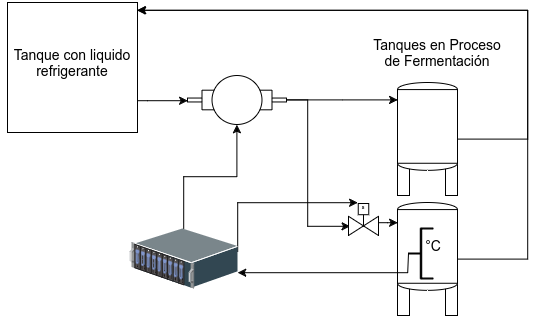
\includegraphics[width=.8\textwidth]{./imagenes/diagrama_del_sistema.png}}
  \end{figure}	
  \vspace{-55px}
  \hspace{25px}\small\color{black}{Dispositivo}\\
  \hspace{20px}\small\color{black}{Implementado}
\end{frame}


\begin{frame}{\textbf{\LARGE{Planificación del proyecto }}}
  \fontsize{18pt}{18}\selectfont
  \begin{itemize}
    \item Análisis del Proyecto
      \vspace{10px}
    \item Hardware
      \vspace{10px}
    \item Software
      \vspace{10px}
    \item Plataforma web
      \vspace{10px}
    \item Informes y conclusiones
  \end{itemize}	
\end{frame}


\subsection{Hardware}
\begin{frame}{\textbf{\LARGE{CIAA-NXP}}}
  \vspace{-.7cm}
  \begin{figure}[H]
    {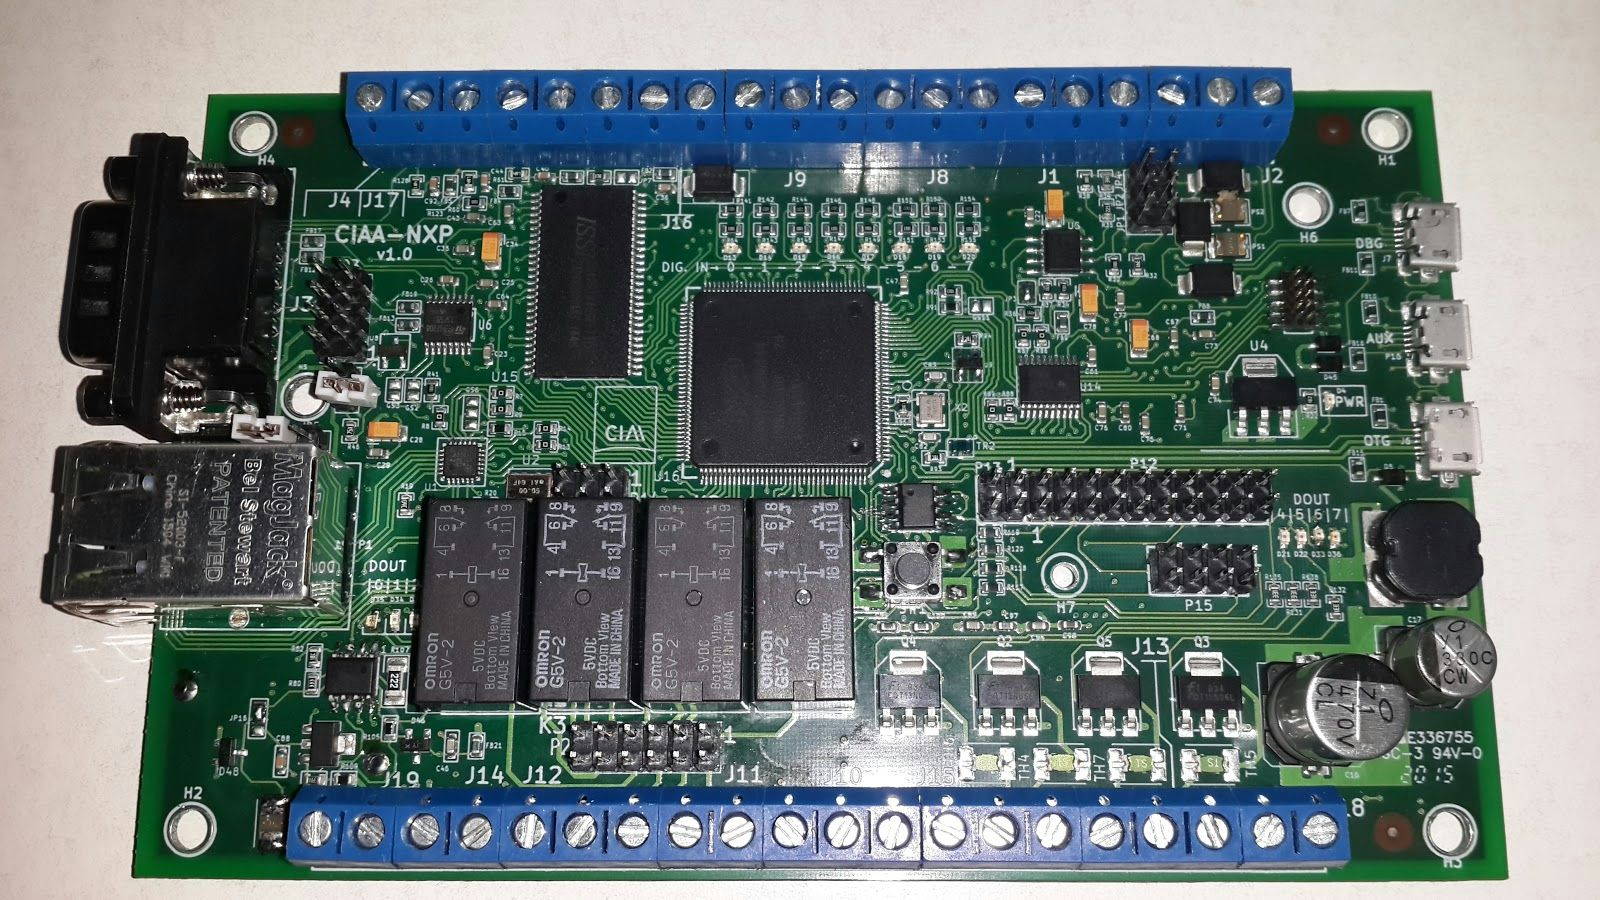
\includegraphics[width=1\textwidth]{./imagenes/ciaa.png}}
  \end{figure}	
\end{frame}

\begin{frame}{\textbf{\LARGE{Diseño simulador del sistema}}}
  \vspace{-.7cm}
  \begin{figure}[H]
    {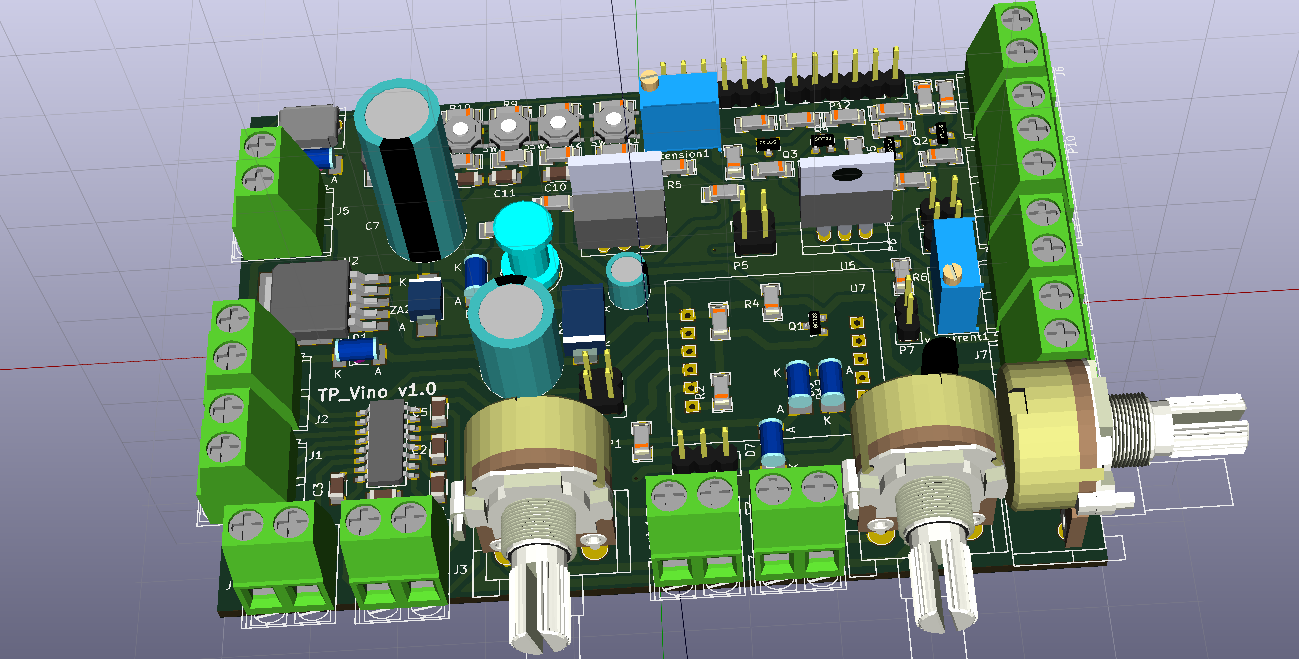
\includegraphics[width=1\textwidth]{./imagenes/pcb_3d.png}}
  \end{figure}	
\end{frame}

\begin{frame}{\textbf{\LARGE{Prototipo experimental}}}
  \vspace{-.7cm}
  \begin{figure}[H]
    {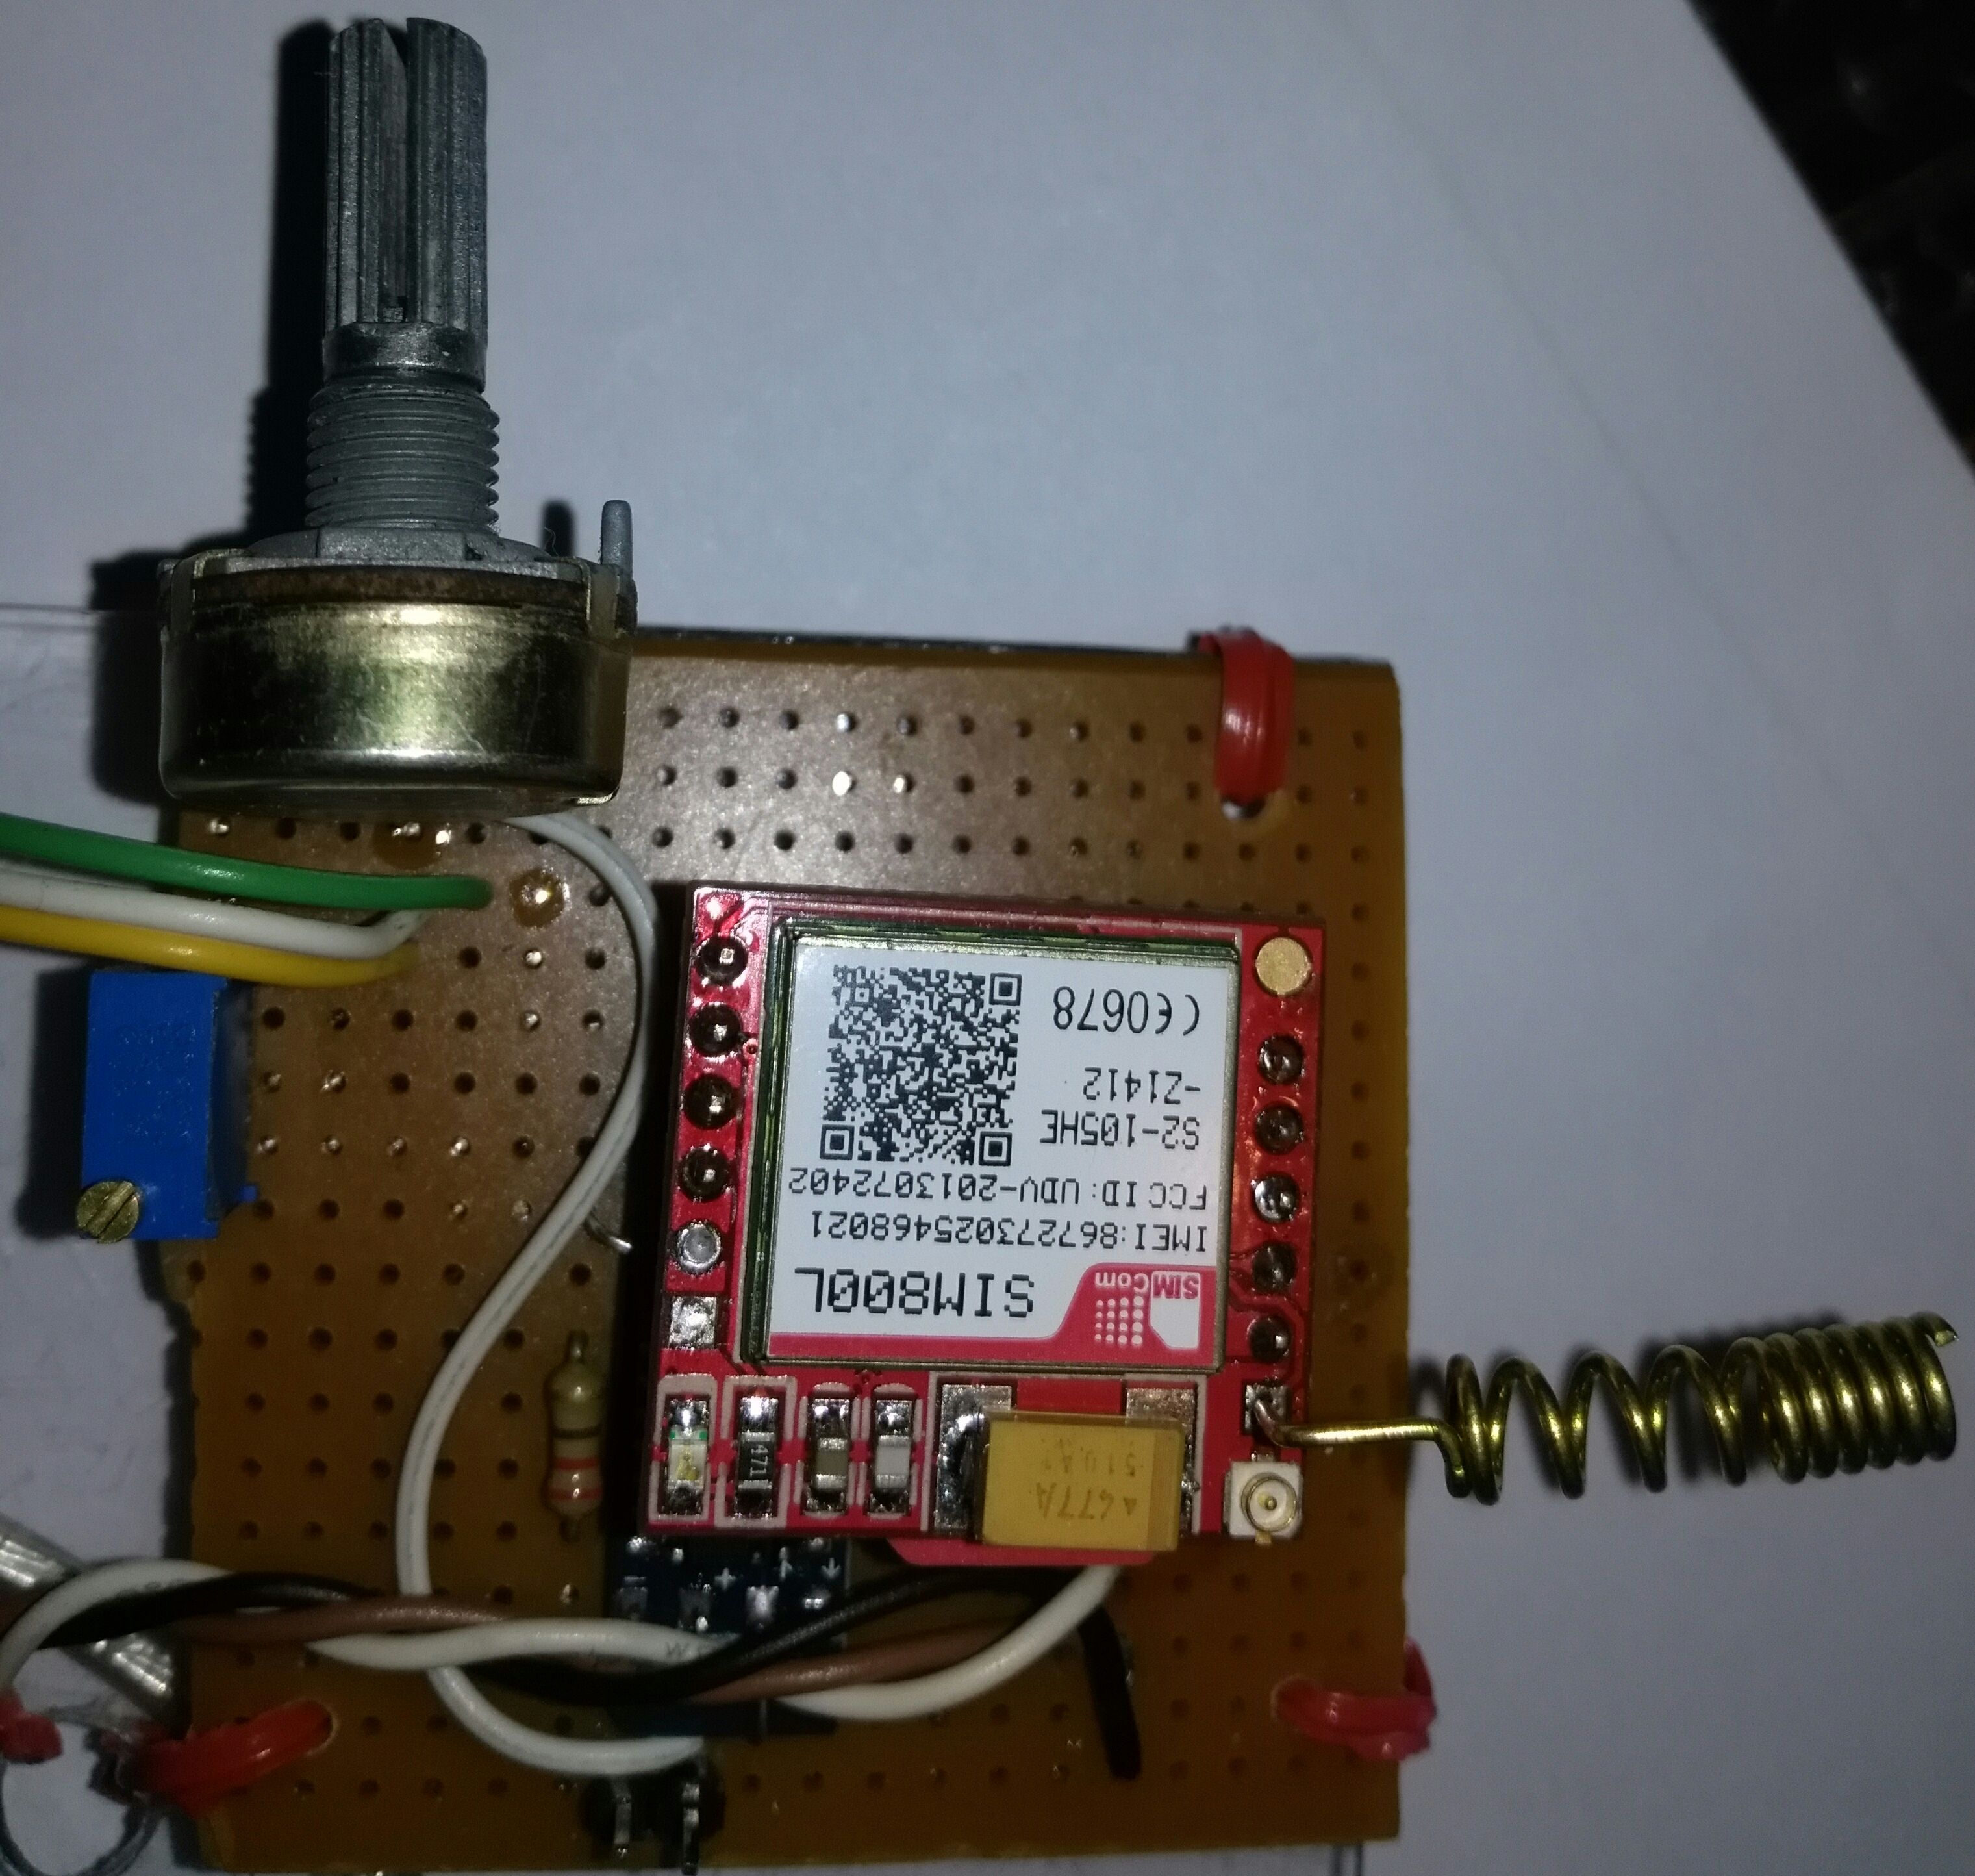
\includegraphics[width=.5\textwidth]{./imagenes/placa_basica.jpg}}
  \end{figure}	
\end{frame}

\subsection{Software}
\begin{frame}{\textbf{\LARGE{Software}}}
  \fontsize{18pt}{18}\selectfont
    \begin{itemize}
      \item Proyecto CIAA Firmware
      \vspace{15px}
      \item Real Time Operating System (RTOS)
      \vspace{15px}
      \item LwIP
    \end{itemize}

\end{frame}


\subsection{Plataforma Web}

\begin{frame}{\textbf{\LARGE{Tecnologías Utilizadas}}}
  \fontsize{18pt}{18}\selectfont
  \begin{itemize}
    \item Webserver HTTP 2.0
      \vspace{10px}
    \item JavaScript
      \vspace{10px}		
    \item Server Side Includes (SSI)
      \vspace{10px}
    \item Asynchronous JavaScript and XML (AJAX)
      \vspace{10px}
    \item Common Gateway Interface (CGI)
  \end{itemize}
\end{frame}

\begin{frame}{\textbf{\LARGE{Interfaz Web}}}
  \vspace{-.7cm}
  \begin{figure}[H]
    {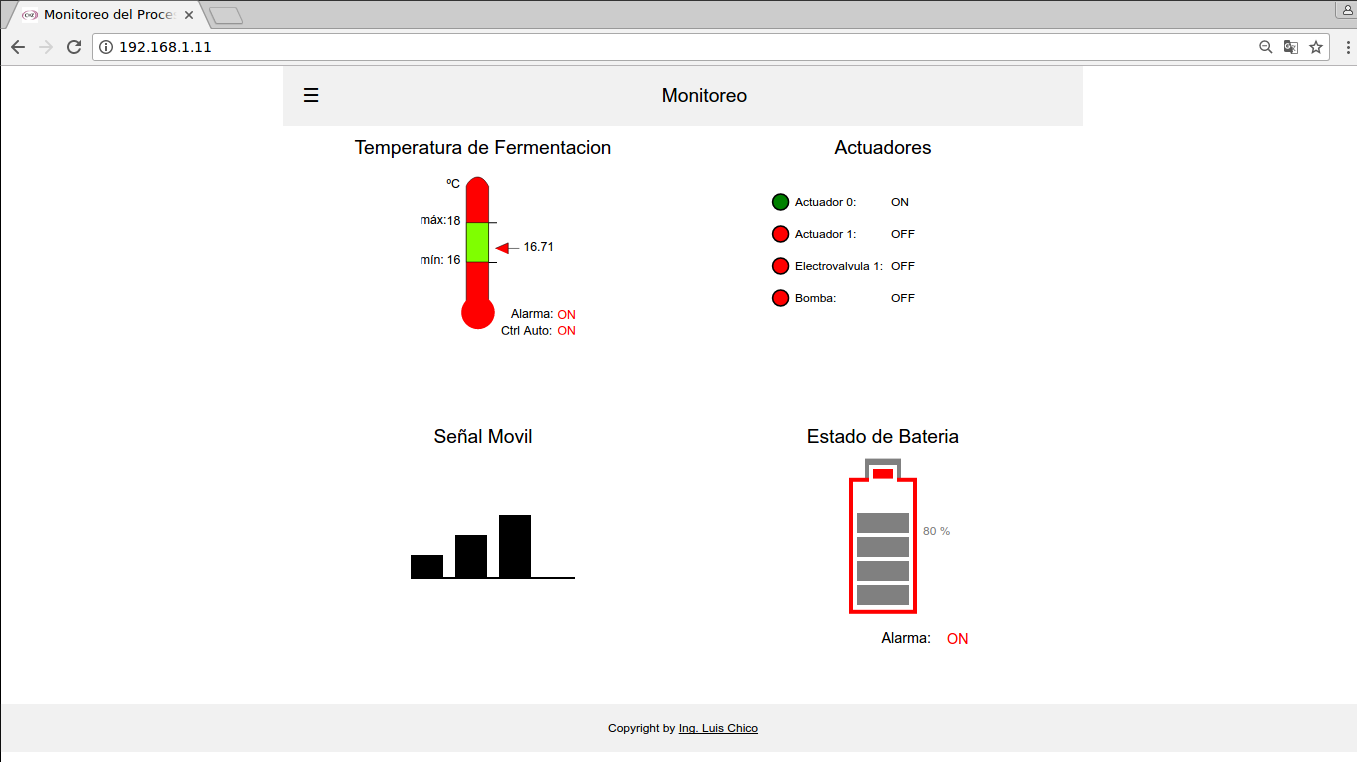
\includegraphics[width=1\textwidth]{./imagenes/web_monitoreo.png}}
  \end{figure}	
\end{frame}

\begin{frame}{\textbf{\LARGE{Menus de Configuración}}}
  \vspace{-.7cm}
  \begin{figure}[H]
    {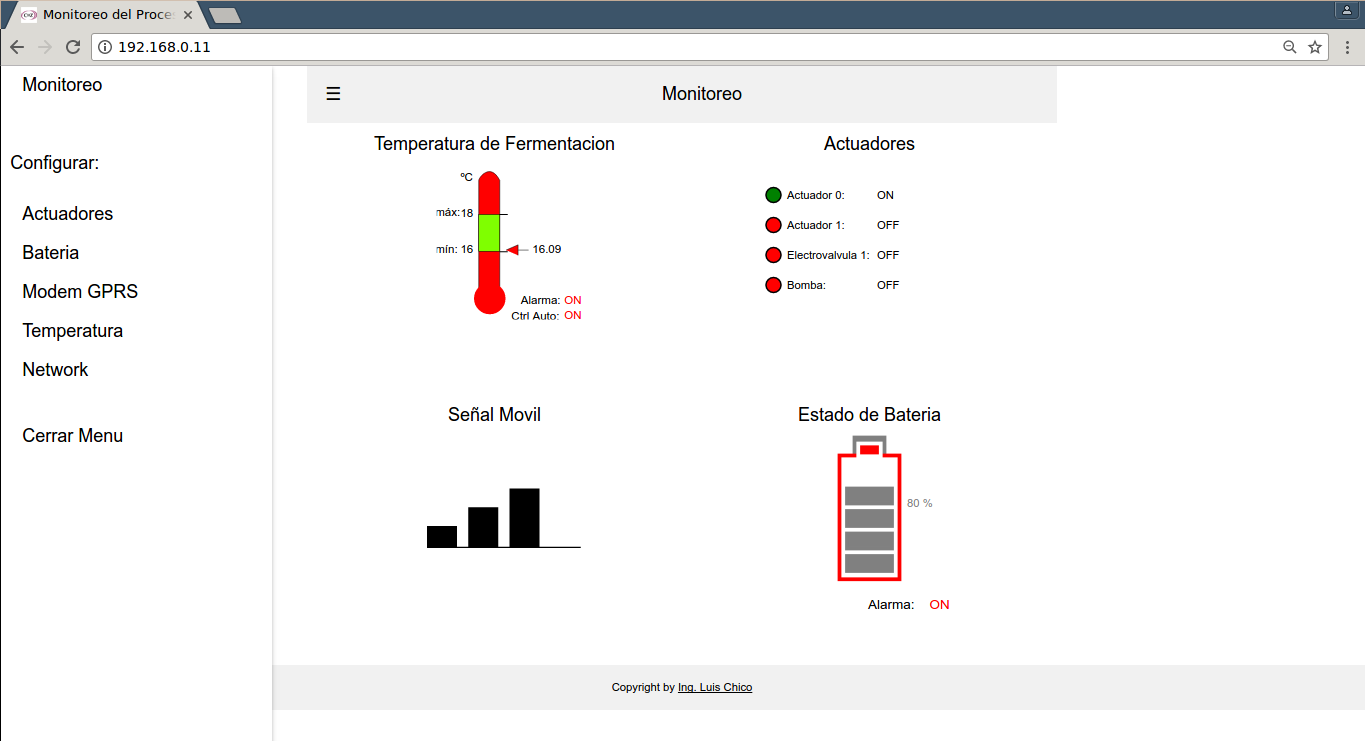
\includegraphics[width=1\textwidth]{./imagenes/web_menus.png}}
  \end{figure}	
\end{frame}

\begin{frame}{\textbf{\LARGE{Configuración de Temperatura}}}
  \vspace{-.7cm}
  \begin{figure}[H]
    {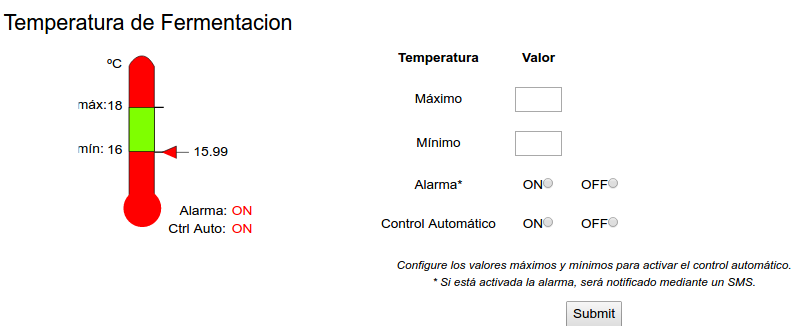
\includegraphics[width=1\textwidth]{./imagenes/config_temp.png}}
  \end{figure}	
\end{frame}

\begin{frame}{\textbf{\LARGE{Configuración de Actuadores}}}
  \vspace{-.6cm}
  \begin{figure}[H]
    {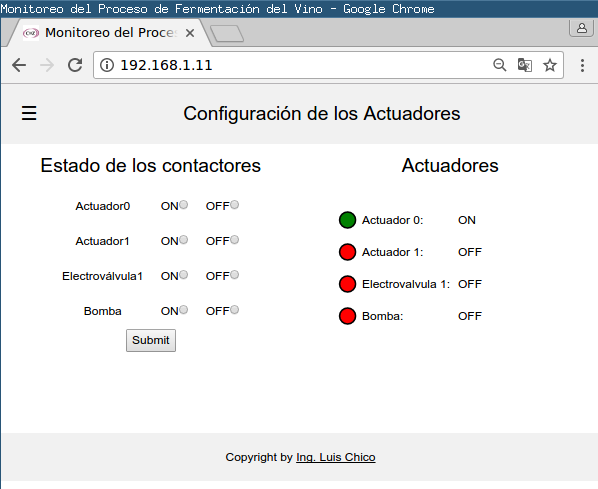
\includegraphics[width=0.8\textwidth]{./imagenes/config_act.png}}
  \end{figure}	
\end{frame}

\begin{frame}{\textbf{\LARGE{Configuración de Contactos}}}
  \vspace{-.7cm}
  \begin{figure}[H]
    {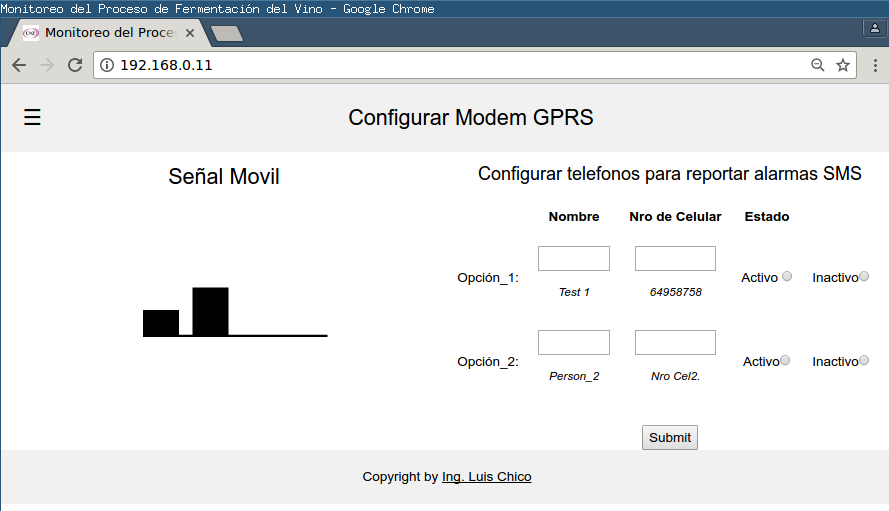
\includegraphics[width=1\textwidth]{./imagenes/config_Modem.png}}
  \end{figure}	
\end{frame}

\begin{frame}{\textbf{\LARGE{Alarma por consumo de Batería}}}
  \vspace{-.7cm}
  \begin{figure}[H]
    {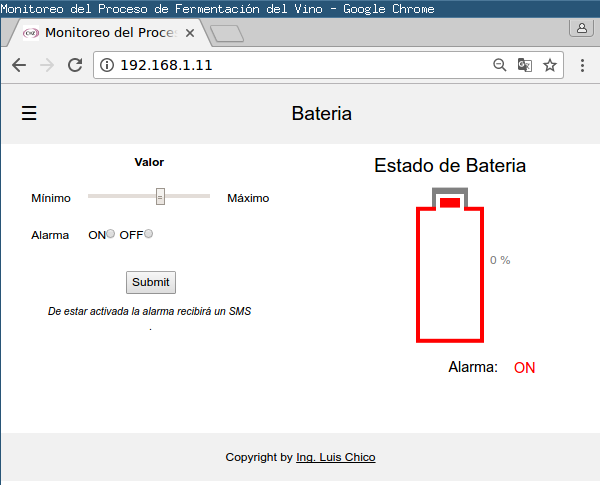
\includegraphics[width=0.8\textwidth]{./imagenes/config_bat.png}}
  \end{figure}	
\end{frame}

\begin{frame}{\textbf{\LARGE{Configuración de la Red}}}
  \vspace{-.7cm}
  \begin{figure}[H]
    {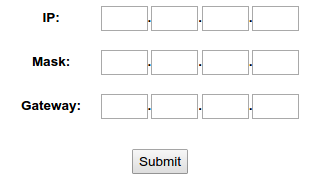
\includegraphics[width=1\textwidth]{./imagenes/config_network.png}}
  \end{figure}	
\end{frame}

\section{Conclusiones}

\begin{frame}{\textbf{\LARGE{Conclusiones}}}
  \fontsize{16pt}{16}\selectfont
  \begin{itemize}
    \item Realizar un control manual y automático del sistema
      \vspace{10px}
    \item Se aplicaron los conocimientos adquiridos en la carrera para obtener un sistema embebido sobre la CIAA-NXP.
      \vspace{10px}
    \item Permite acceder mediante una página web al estado del sistema.
  \end{itemize}
\end{frame}

\begin{frame}{\textbf{\LARGE{Trabajo Futuro}}}
  \fontsize{16pt}{16}\selectfont
  \begin{itemize}
    \item Ampliar la capacidad de control a cuatro tanques.
      \vspace{15px}
    \item Ampliar las funcionalidades de los SMS, para consultas y posibles controles. 
      \vspace{15px}
    \item Agregar retroalimentación de sensores y actuadores por hardware para un control más robusto.
      \vspace{15px}
    \item Adicionar una opción de control por intervalos de tiempos. 
  \end{itemize}
\end{frame}

\begin{frame}{\textbf{\LARGE{Gracias por su atención!}}}
      \begin{figure}[H]
        {
\includegraphics[width=.5\textwidth,clip,trim=2cm 5cm 3cm 2cm]{./imagenes/gracias.jpg}}
      \end{figure}	
\end{frame}

\end{document}
